\documentclass[12pt]{article}


\usepackage{scicite}
\usepackage{hyperref}
\usepackage{graphicx}
\usepackage{caption} 
\usepackage{subfigure}
\usepackage{float}
\usepackage{amsmath}
\usepackage{amssymb}
\usepackage{times}
\usepackage{listings}


\topmargin 0.0cm
\oddsidemargin 0.2cm
\textwidth 16cm 
\textheight 21cm
\footskip 1.0cm



\newenvironment{sciabstract}{%
\begin{quote} \bf}
{\end{quote}}



\renewcommand\refname{References and Notes}


\newcounter{lastnote}
\newenvironment{scilastnote}{%
\setcounter{lastnote}{\value{enumiv}}%
\addtocounter{lastnote}{+1}%
\begin{list}%
{\arabic{lastnote}.}
{\setlength{\leftmargin}{.22in}}
{\setlength{\labelsep}{.5em}}}
{\end{list}}



\title{Deep speech} 


\author
{Vincent R\'ebiscoul, St\'ephane Pouget and Florent Gu\'epin}


\date{}






\begin{document} 

% Double-space the manuscript.

\baselineskip24pt

% Make the title.

\maketitle 



% Place your abstract within the special {sciabstract} environment.

\begin{sciabstract}
  This document present our project in machine learning. We have implemented a voice recognition system i.e. our program is able to recognize spoken language and translate into text by using computers.
 We use python3, Keras and Tensorflow.
\end{sciabstract}

\begin{figure}[H]
  \begin{center}
    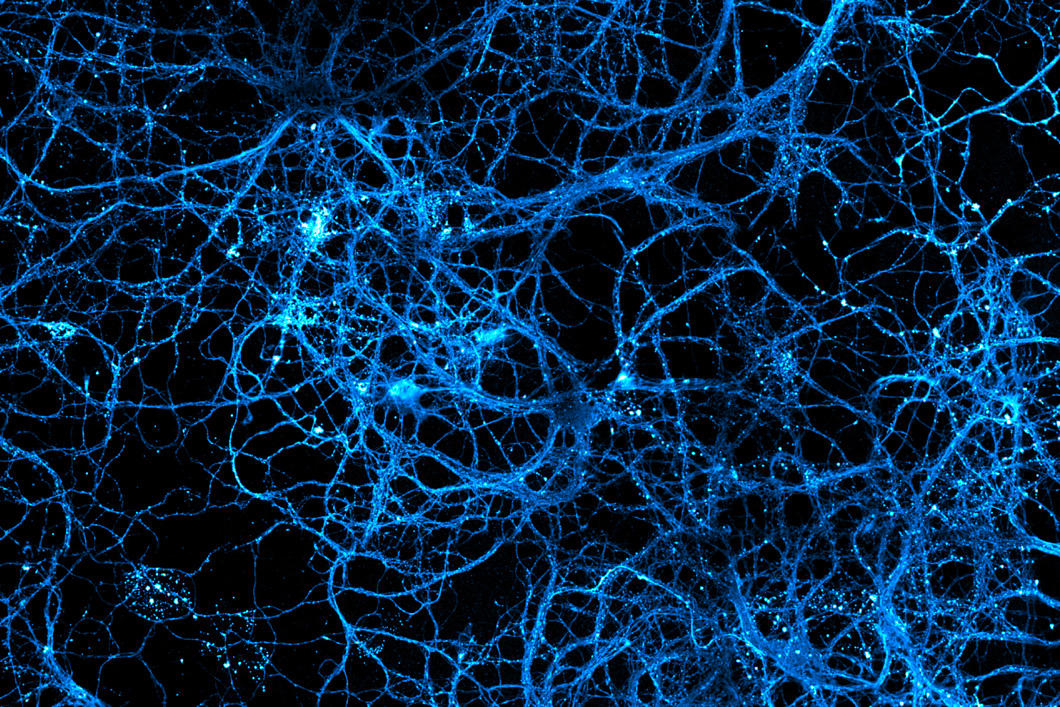
\includegraphics[scale=0.30]{images/neu.jpg}
    \caption{Neurons}
  \end{center}
\end{figure}

\newpage


\section*{Introduction}

We have implemented this article \cite{article} with Python3, Keras and Tensorflow. The neural network used is not common (it is a non-sequential recurrent neural network). So we created our own neural network model using Keras.

\section{Model}

\subsection{Topology of the model}

The core of the system is a recurrent neural network trained to ingest speech spectrograms and to generate English text transcriptions.

Let a single utterance $x$ and label $y$ be sampled from a
training set $X = \{(x^{(1)}, y^{(1)}), (x^{(2)}, y^{(2)}), . . .\}. $ Each utterance, $x^{(i)}$, is a time-series of length $T^{(i)}$
where every time-slice is a vector of audio features, $x^{(i)}$ ,$ t = 1, . . . , T^{(i)}$ . We use spectrograms as our features, so $x^{(i)}_{t,p}$ denotes the power of the $p$’th frequency bin in the audio frame at time t. The goal of our RNN is to convert an input sequence $x$ into a sequence of character probabilities for the transcription $y$, with $ \hat{y}= \mathbb{P}(c_t |x),$ where $c \in \{a,b,c, . . . , z, space, apostrophe, blank\}.$

We have five layers of neurons. The three first layers are computed by:

\[ h_t^{(l)} = g(W^{(l)}h_t^{(l-1)} + b^{(l)}) \]

where $g(z) =$ min\{max $\{0,z\}, 20\}$ and $W^{(l)}, b^{l}$ are the matrix weights and bias parameters for layer $l$.

The fourth layer is a bi-directional recurrent layer. This layer includes two sets of hidden units : a set with forward recurrence, $h^{(f)}$, and a set with backward recurrence $h^{(b)}$ : 

\[ h_t^{(f)} = g(W^{(4)}h_t^{(3)} + W_r^{(f)}h_{t-1}^{(f)} + b^{(4)}) \]

\[ h_t^{(b)} = g(W^{(4)}h_t^{(3)} + W_r^{(b)}h_{t+1}^{(b)} + b^{(4)}) \]

The fifth (non-recurrent) layer takes both the forward and backward units as inputs $h_t^{(5)} = g(W^{(5)}h_t^{(4)} + b^{(5)} $ where $h_t^{(4)} = h_t^{(f)} + h_t^{(b)}$. The output layer is a standard softmax function that yields the predicted character probabilities for each time slice $t$ and character $k$ in the alphabet :

\[ h_{t,k}^{(6)} \equiv \mathbb{P}(c_t=k | x) = \frac{exp(W_k^{(6)}h_t^{(5)} + b_k^{(6)})}{\sum_j exp(W_j^{(6)}h_t^{(5)} + b_j^{(6)})} \]


\begin{figure}[H]
  \begin{center}
    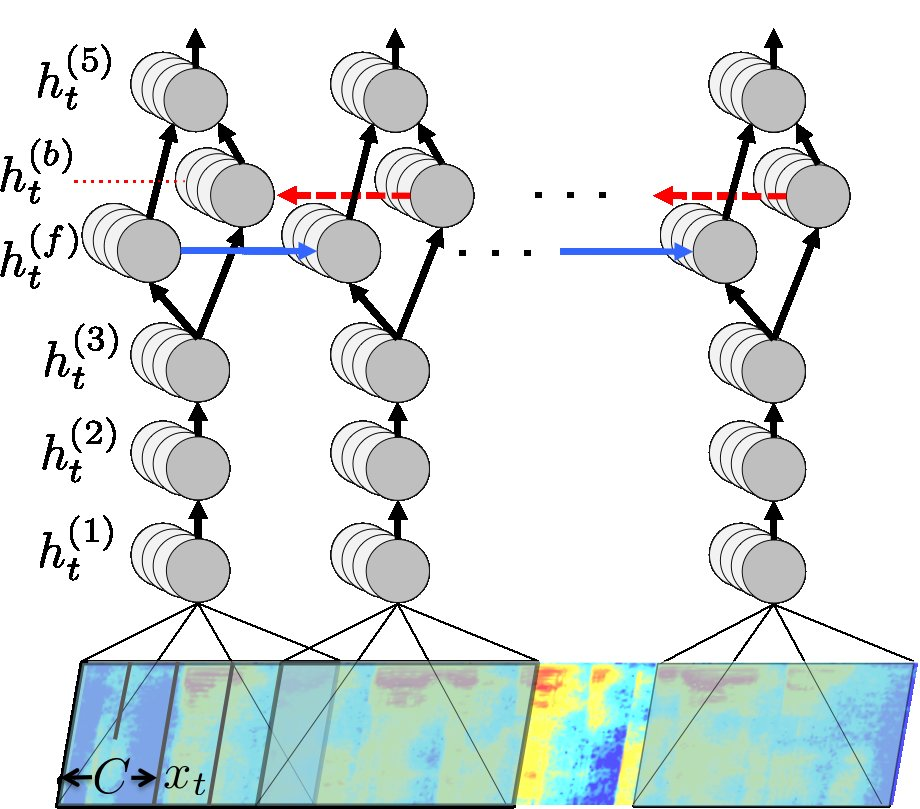
\includegraphics[scale=0.27]{images/photo.jpg}
    \caption{Structure of our RNN model}
  \end{center}
\end{figure}

\subsection{Analysis of the model}
The model we use is a Recurrent Neural Network (RNN), the particularity of a recurrent neural network is that recurrent layers have a state and to compute the value of a time slice, the layer can take the output value of the same layer one step before or one step after. In our case, we have two recurrent layers, with $h_t^f$ depends on $t-1$ (so $h_t^f$ depends on what happened previously). $h_t^b$ depends on $t+1$ so it depends on what happen next, in the spectrogram. The idea is that we cannot link a sound to a letter without putting it in context. For example, in the word "the", a non recurrent neural network cannot predict that the first letter is t because t has several pronunciation depending on the letter preceding or following. This is why we need two recurrent layers, one with a forward recurrence and one with a backward recurrence.


\section{Our work}

\subsection{The implementation of the model}

This article \cite{article} creates a new model and use a CTC loss function. So to create this model, we have customized our model so that it is like on the article. For that we had to work a lot on the documentation of Keras and Tensorflow. However our main problem was the CTC loss function. At the beginning, we had trouble to understand how the backend function ctc\_batch\_ cost worked. First, one has to know that the CTC loss function is very peculiar. Indeed, our neural network slices an audio file in several time slices and then for each time slice, it tries to predict which letter it is. Now, suppose you give a recording of someone saying the expression ``good morning''. If the neural network is correctly trained, it should output something like ``gggoooodd moorrnnninng'' (there are several time slices corresponding to the same letter), thus the cost $\mathcal{L}(\mbox{good morning}, \mbox{gggoooodd moorrnnninng})$ should be small when the cost $\mathcal{L}(\mbox{good morning}, \mbox{good mornint})$ should be higher. This makes the CTC function essential but complicated. Another problem is that the ctc\_batch\_cost function takes four parameters, but in Keras, the loss function only takes 2 parameters. To avoid this problem, we had to create a new lambda layer which outputs the loss of the batch and is connected to several other layers which feeds the different arguments that are needed. Apparently, this is a known trick in Keras to avoid this common problem. \\

Our model is implemented like this :

\begin{lstlisting}
h1 = TimeDistributed(Dense(128, activation=clipped_relu))(inputs)
h2 = TimeDistributed(Dense(128, activation=clipped_relu))(h1)
h3 = TimeDistributed(Dense(128, activation=clipped_relu))(h2)


lb = GRU(128, go_backwards = True, return_sequences = True)(h3)
lf = GRU(128, return_sequences = True)(h3)


h4 = Add()([lb,lf]) # add the two layers

h5 = TimeDistributed(Dense(128, activation=clipped_relu))(h4)
h6 = TimeDistributed(Dense(29, activation='softmax'),name='aux_output')(h5)
\end{lstlisting}

\subsection{The dataset}

The dataset that we used is not composed of sentences or expressions but of words. The idea was to have an easily trainable neural network that could work quickly and would be able to recognize at least some words. Indeed, in the article they say they managed to have a solid working neural network but using several optimization and with 5000+ hours of training. This seemed too much for machine learning rookies. Obviously this makes a neural network weak when you train it on sentences but it works better on words (at least the words where the neural network has been trained on).

\subsection{Our results}

\begin{figure}[H]
  \begin{center}
    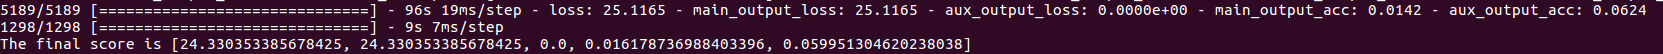
\includegraphics[scale=0.4]{images/image2.png}
    \caption{Result after a training of 4 epochs}
  \end{center}
\end{figure}


\begin{figure}[H]
  \begin{center}
    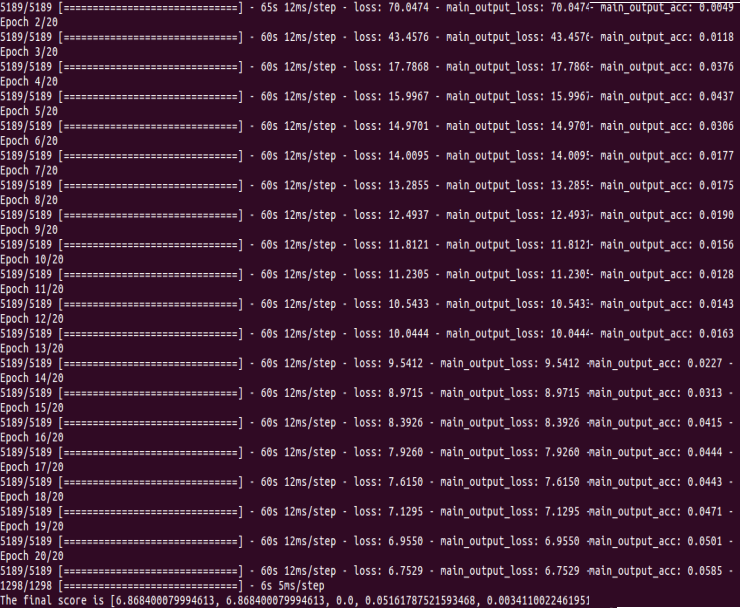
\includegraphics[scale=0.80]{images/image3.png}
    \caption{Result after a training of 20 epochs}
  \end{center}
\end{figure}

This were 2 examples of a training session of our neural network. On the second one, several interesting things happened, we can notice : our neural network is able to learn efficiency after the 12th epochs, before he is not able to distinguish efficiently. We also have to make a test over more epochs (something like 200), to see a good learning from our neural network. 
Here, we used 3 words, with more than 5100 files. At the end, our neural network is able to know 5/100 words of people. It's pretty bad for a neural network, but it is only with 20 epochs! 
With 85 epochs, our neural network have a loss of 4 and he is able to recognize 15 words out of 100, which is not bad. Unfortunately, working and training the neural network on CPU takes a while, and we could not make more epochs (with 85 epochs, it took 2 hours to compute)

The training is on 3 words, out of 30. We made our neural network such that he have to load everything (meaning 5198 files ..) on memory before attempting to compute. We could have make it differently : loading the files during he computation. But we did not manage to do it.

Something interesting to quote is also that the accuracy, during the training of our neural network, is serrated increasing : during the first 4 epochs it increase, then it decreases to 0, and increases again at epochs 13, to go further the top lvl of the 4th epoch, to decrease after, again and again. 


\newpage
\section{Conclusion}

This was an interesting experience, however we ran into several problems and it was very painful to correct them. Indeed, making a non-trivial RNN is hard when you go not discover Machine Learning. There are fewer examples on the internet and it makes the model hard to optimize. Indeed, the article proposes several optimization (like doing computations in parallel) but we had no time to try them because it seemed to be for ML experts.

Also, our neural network is hard to use to translate an audio file to text (which is the whole point), we think the problem is that we did not train our RNN enough, but it takes a lot of time and maybe our dataset was not large enough? We think we made mistakes on how we designed our program. For example, at the beginning, the program loads all the data and then it starts to learn. The problem is that we have a very limited amount of RAM when it comes to learning from audio files. Thus, we need to think how we could go around that. Also, when we get the spectrogram of a file, we can choose the size of the frequency sampling, maybe we could have used a greater value but then, the computations would have been very long.

However, this was interesting to do, we understood how you had to test several parameters to finally have a satisfying result. Nevertheless, this can be frustrating because you never know if your model is a good one because one cannot predict the right combination of model/parameters in advance.

\newpage
\bibliography{scicite}

\bibliographystyle{Science}

\end{document}